\subsection{Rasterisierung}
\label{sec:Rasterisierung}
Um ein Rasterbasiertes Modell wie ConvLSTM oder ST-ResNet für die Vorhersage von mobilen Radarkontrollen verwenden zu können, müssen die räumlich und zeitlich kontinuierlichen Datenpunkte aus dem Datensatz zunächst rasterisiert werden.
Dazu ist es sinnvoll nochmals zu betrachten, wie die Daten ursprünglich vorliegen.
Jede Meldung ist eine Zeile in einer Datenbanktabelle mit den Spalten \emph{Längengrad}, \emph{Breitengrad}, \emph{Aufbauzeitpunkt} und \emph{Abbauzeitpunkt}.
Das Ziel besteht darin, die Datenpunkte so zu verarbeiten, dass pro Zeitraum $T$ ein Raster aus $n \times n$ quadratischen Zellen mit der Seitenlänge $k$ entsteht, bei dem jeder Zelle ein Wert $x$ zugeordnet ist, der etwas über die gemeldeten Radarkontrollen in dieser Zelle aussagt.
Die Werte $T,~n,~k$ sind hierbei variable Hyperparameter und müssen möglichst sinnvoll ausgewählt werden.
Außerdem muss festgelegt werden, nach welcher Regel der Wert $x$ berechnet werden soll.
Bei der Auswahl des Zeitraums $T$ muss zwischen der gewünschten zeitlichen Genauigkeit und der Anzahl an verfügbaren Datenpunkten abgewägt werden.
Wird $T$ beispielsweise zu klein gewählt, enthält der betrachtete Bereich zu wenige Meldungen, um auf deren Basis aussagekräftige Vorhersagen treffen zu können.
Wird $T$ hingegen zu groß gewählt (wie z. B. eine Woche oder ein Monat), haben die Vorhersagen weniger praktischen Nutzen.
Außerdem könnten dann insgesamt zu wenige Zeitschritte vorliegen, um das Modell trainieren zu können.
Nach einigen Versuchen scheinen 24 Stunden für $T$ ein guter Wert zu sein, da somit der praktische Nutzen erhalten bleibt und es dennoch genug Meldungen pro Zeitschritt gibt.

Als nächstes sind $k$ udn $n$ zu wählen.
Die Seitenlänge des gesamten betrachteten Bereichs berechnet sich daraus mit $n \cdot k$.
Bei der Wahl von $k$ muss dieselbe Abwägung getroffen werden wie bei der Wahl von $T$, jedoch geht es hier um den praktischen Nutzen der Vorhersagen je nach räumlicher Auflösung.
Wird $k$ zu groß gewählt, ist die zeitliche Auflösung zu gering, als dass die Vorhersagen nützlich wären.
Wenn $k$ hingegen zu klein gewählt wird, gibt es in zu wenigen Zellen eine Meldung, um das Modell gut trainieren zu können.
Bei der Wahl von $k$ kommt es außerdem darauf an, ob eher städtischer oder ländlicher Raum betrachtet werden soll.
Für den ländlichen Raum scheint $k = 4~\text{km}$ eine gute Wahl zu sein, da die Radarkontrollen dort nicht sonderlich dicht liegen.
Für den städtischen Raum ist dieser Wert jedoch eher zu groß, da sich in einem 4 km Radius vergleichsweise deulich mehr Straßen befinden.
Außerdem ist die Dichte an Radarkontrollen im städtischen Raum höher, weshalb ein geringeres $k$ von einem oder zwei Kilometer durchaus möglich ist.
Wird (beispielsweise in Baden-Württemberg) insgesamt ein größerer Raum abgedeckt, besteht die meiste Fläche aus ländlichem Gebiet.
Daher wird im folgenden mit $k = 4~\text{km}$ fortgefahren.
Die Wahl von $n$ beeinflusst nun den insgesamt durch das Raster abgedeckten Raum.
Optimalerweise sollte dieser Wert möglichst groß sein, um möglichst viele Trainingsdaten einzuschließen.
Andererseits ist $n$ durch den währen des Trainings verfügbaren Speicher begrenzt.
Wird das Training auf einer Grafikkarte ausgeführt, muss das komplette Modell und alle Trainingsdaten, die pro Batch verarbeitet werden in den Grafikspeicher passen.
Da der Speicherbedarf quadratisch mit $n$ ansteigt, ist man hier in der Praxis sehr eingeschränkt.
Bei einem Grafikspeicher von 8 GB und einer Batch Size von 12 ist $n = 50$ gut möglich.
Mit $k = 4~\text{km}$ ergibt sich dann eine Seitenlänge des gesamten Rasters von 200 km.

Für die Berechnung von $x$ gibt es mehrere Möglichkeiten.
Zunächst könnte $x = 1$ gesetzt werden, wenn sich in der Zelle mindestens eine Radarkontrolle befindet, ansonsten $x = 0$.
Alternativ kann $x$ auf die Anzahl der Radarkontrollen gesetzt werden, die sich im jeweiligen Zeitraum in der Zelle befinden.
Dies hat jedoch den Nachteil, dass eine Radarkontrolle mit einer kurzen Standdauer gleich gewichtet wird wie eine Radarkontrolle mit einer deutlich längeren Standdauer.
Daher bietet es sich an, die Standdauer aller Radarkontrollen in einer Zelle aufzusummieren.
Mit dieser Möglichkeit enthält $x$ am meisten Informationen über die Radarkontrollen in der jeweiligen Zelle.
Außerdem kann diese Repräsentation auch nach der Rasterisierung einfach in eine binäre Unterscheidung umgewandelt werden, indem pro Zelle $x := x > 0$ gesetzt wird.

Nun stellt sich die Frage, wie die Rasterisierung mit den erörterten Parametern möglichst effizient ausgeführt werden kann.
Die einfachste Möglichkeit besteht darin, alle Meldungen pro Rasterzelle und Datum nacheinander mit einem Python-Skript von der MariaDB-Datenbank abzufragen.
Pro Rasterzelle dauert diese Abfrage ca. 0,32 Sekunden.
Bei 200 Zellen und 2648 Tagen würde die Rastergenerierung damit jedoch 47 Stunden dauern, was unpraktikabel ist.
Eine mögliche Optimierung ist, eine Geodatenbank zu verwenden, die das Filtern nach Koordinaten effizienter ausführen kann als MariaDB.
Eine solche Geodatenbank ist PostgreSQL mit der Erweiterung PostGIS.
Die Abkürzung \acrshort{gis} in PostGIS steht für \acrlong{gis}.
Dies ist ein Begriff für Systeme, die besonders auf die Verarbeitung von räumlichen Daten optimiert sind, wozu auch Geodatenbanken gehören.
Eines der wichtigsten Features einer Geodatenbank ist ein räumlicher Index (engl. \emph{spatial index}).
Ein solcher ist laut \cite[S. 2707 f.]{SpatialIndexingTechniques} eine Datenstruktur, die einen schnelleren Zugriff auf räumliche Daten bietet als traditionelle eindimensionale Indexe wie ein B\textsuperscript{+}-Baum.
Ein bekanntes Beispiel für einen räumlichen Index ist der R-Baum, der auch von PostGIS verwendet wird \cite{PostGISSpatialIndex}.
Die Funktionsweise eines R-Baums ist in \autoref{fig:RTreeImage} dargestellt.

\begin{figure}[h]
    \centering
    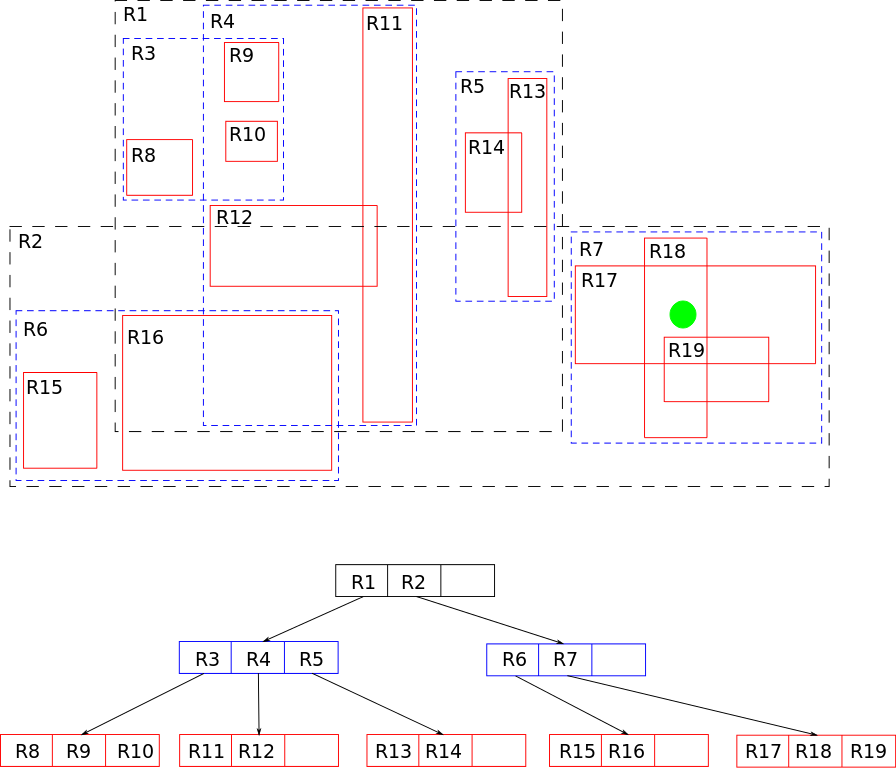
\includegraphics[width=1.0\textwidth,height=10cm,keepaspectratio=true]{content/images/R-tree.png}
    \caption{Aufbau und Funktionsweise eines R-Baums \cite{RTreeImage}}
    \label{fig:RTreeImage}
\end{figure}

Wie in der Abbildung zu erkennen ist, enthält jeder Knoten eines R-Baums Informationen über ein Rechteck.
Die Knoten können dann nach \cite{RTrees} jeweils Kindknoten haben, deren Recktecke komplett innerhalb des Rechtecks des Elternknotens liegen müssen.
Als Beispiel für die Suchoperation auf einem R-Baum sollen alle Rechtecke R8 bis R19 ermittelt werden, die sich mit dem in \autoref{fig:RTreeImage} grün markierten Punkt überschneiden.
Ohne den R-Baum müssten alle 12 Recktecke R8 bis R19 nacheinander mit dem Punkt verglichen werden.
Mit dem R-Baum sind nur noch sieben Vergleiche notwendig.
Zunächst wird ermittelt, ob der Punkt in R1 oder R2 liegt.
Da der Punkt in R2 liegt, können R8 bis R14 nun schon ausgeschlossen werden.
Daraufhin wird der Punkt mit R6 und R7 verglichen.
Da der Punkt in R7 liegt, liefern die Vergleiche mit R17, R18 und R19, dass sich nur R17 und R18 mit dem Punkt überschneiden.
Dieser Performancegewinn macht sich nach \cite{RTrees} vor allem bei sehr vielen Datenpunkten bemerkbar.

Da der Datensatz der Mobilen Radarkontrollen ca. 7,7 Millionen Einträge enthält, ist es hier sehr sinnvoll, eine Geodatenbank mit räumlichem Index zu verwenden.
Als Geodatenbank bietet sich PostgreSQL mit der PostGIS-Erweiterung (im folgenden zusammen PostGIS genannt) an.
Die Datenpunkte müssen nun von MariaDB nach PostGIS übertragen werden.
Dies kann komfortabel mit einem Python-Skript unter Verwendung der Pakete SQLAlchemy und GeoAlchemy2 bewerkstelligt werden.
Mit SQLAlchemy kann intuitiv auf Datenbanken zugegriffen werden, indem Tabellen der Datenbank auf Python-Klassen abgebildet sind.
Dieses Konzept wird als \acrfull{orm} bezeichnet \cite{SQLAlchemyKeyFeatures}.
Das Paket GeoAlchemy2 fügt dann noch Unterstützung für PostGIS hinzu.
Nun können zwei Klassen entworfen werden, die eine Radarkontrolle in MariaDB und in PostGIS repräsentieren.
Die Implementierung der beiden Klassen und des letztendlichen Transfers ist in \appendixref{sec:ToPostGIS} zu finden.
Die Klasse \emph{PostgisSpeedcam} enthält dabei einen Konstruktor, der eine MariaDB-Radarkontrolle als Parameter erhält und die Konvertierung durchführt.
Mit der Implementierung in \autoref{lst:ToPostGIS} können alle Tabelleneinträge in ca. einer Stunde übertragen werden.
Hierbei ist wichtig anzumerken, dass der räumliche Index automatisch von PostGIS erzeugt und aktualisiert wird.

Die Verwendung von PostGIS bringt noch einen weiteren großen Vorteil mit sich.
Da die Daten nun in einem im \acrshort{gis}-Umfeld gebräuchlichen Format vorliegen, können beliebige \acrshort{gis}-Tools verwendet werden, um die Daten zu analysieren.
Dies hat den Vorteil, dass diese Tools viele effiziente Implementierungen der Standardalgorithmen auf geographischen Daten mitbringen.
Ein Beispiel für ein solches Tool ist QGIS.
QGIS kann als Algorithmensammlung für geographische Daten angesehen werden.
Außerdem beinhaltet QGIS eine \acrfullr{gui}, mit der diese Algorithmen ausgeführt werden können.
Mit der \acrshort{gui} können zudem verschiedenste geographische Daten wie Punkte, Linien, Rechtecke, Raster etc. visualisiert werden, insbesondere auch die Ergebnisse der ausgeführten Algorithmen.
Ein Beispiel für eine Visualisierung mit QGIS ist \autoref{fig:BlitzerMarathonSep2014Vgl}.
Die Punkte werden über eine direkte Verbindung zu PostGIS abgerufen und dann auf einer OpenStreetMap-Karte dargestellt.
Aufgrund des räumlichen Indexes von PostGIS werden die Punkte sehr schnell geladen, insbesondere wenn kleinere Bereiche betrachtet werden.
QGIS ist in C++ unter Verwendung des Qt-Frameworks implementiert.
Die Algorithmen können zusätzlich zur \acrshort{gui} über eine C++ \acrshort{api} aufgerufen werden, für die es auch Python-Bindings gibt.

Für die Rasterisierung des Datensatzes gibt es nun zwei verschiedene Möglichkeiten.
Zum einen könnte die Rasterisierung direkt in der Datenbank mit von PostGIS bereitgestellten \acrshort{sql}-Funktionen durchgeführt werden.
Zum anderen könnten Algorithmen aus QGIS verwendet werden.
Der erste Ansatz hat den Vorteil, dass mit einer Rasterisierung direkt in der Datenbank die maximal mögliche Geschwindigkeit erreichbar wäre.
Allerdings ist zur Implementierung des Algorithmus in \acrshort{sql} ein umfangreiches Fachwissen im \acrshort{gis}-Umfeld erforderlich.
Da \acrshort{gis} an sich ein großer, eigenständiger Forschungsbereich ist, überwiegt dieser Nachteil die eventuell etwas höhere Geschwindigkeit.
Somit fällt die Wahl auf eine Implementierung der Rasterisierung mit Algorithmen aus QGIS.

Für die Implementierung steht zunächst das Erstellen eines Rasters an, also die Berechnung der Grenzen der einzelnen Rasterzellen.
Hierfür kann der QGIS-Algorithmus \emph{Create grid} verwendet werden.
Die wichtigsten Parameter dieses Algorithmus sind die Grenzen des gesamten Rasters (engl. \emph{extent}) und die Seitenlänge der Rasterzellen (oben $k$ genannt).
Die Grenzen des gesamten Rasters müssen anhand von $n$ und $k$ abgeschätzt werden und können in der QGIS-\acrshort{gui} mit der Funktion \emph{Draw on Map Canvas} direkt auf der Karte gezeichnet werden.
